\section{Findings}

\begin{tabular}{lrr}
\toprule
   Alias Name &           \# &          \% \\
\midrule
    \verb|ls| &  \num{83782} &   \num{3.8} \\
    \verb|ll| &  \num{62465} &  \num{2.83} \\
  \verb|grep| &  \num{44479} &  \num{2.02} \\
    \verb|la| &  \num{43760} &  \num{1.99} \\
     \verb|l| &  \num{39539} &  \num{1.79} \\
\bottomrule
\end{tabular}
\hspace{0.3cm}
\begin{tabular}{lrr}
    \toprule
           Command &            \# &           \% \\
    \midrule
        \verb|git| &  \num{327786} &  \num{12.93} \\
         \verb|ls| &  \num{260156} &  \num{10.27} \\
         \verb|cd| &  \num{166632} &   \num{6.58} \\
       \verb|grep| &   \num{89598} &   \num{3.54} \\
        \verb|vim| &   \num{46545} &   \num{1.84} \\
    \bottomrule
\end{tabular}
\hspace{0.3cm}
\begin{tabular}{lrr}
    \toprule
                Argument &            \# &          \% \\
    \midrule
     \verb|--color=auto| &  \num{153931} &  \num{4.24} \\
               \verb|-i| &   \num{70640} &  \num{1.95} \\
               \verb|-a| &   \num{42910} &  \num{1.18} \\
               \verb|-l| &   \num{39519} &  \num{1.09} \\
               \verb|-v| &   \num{35295} &  \num{0.97} \\
    \bottomrule
\end{tabular}



\Cref{tab:top-summary} shows the most common alias names, commands, and arguments appearing in alias definitions.
The most common alias name we found is \texttt{ls}, appearing a total number of \num{83782} times, which is \per{3.8} of all alias definitions.
Note that this is \texttt{ls} as an \emph{alias name}, a redefinition of the \texttt{ls} \emph{command}, which appears \num{260156} times (\per{10.27}).
This is a bit less often than \texttt{git}, the most common command, which appears in \num{327786} aliases (\per{12.93}).
The most common argument, across all commands, is \texttt{--color=auto}, appearing \num{153931} times (\per{4.24})

\newcommand{\numx}[1]{{\small (\num{#1})}}
\begin{table}
    \caption{Top two commands with top arguments and aliases}
    \label{tab:command-summary}
    \begin{tabular}{@{}lrll@{}}
        \toprule
                    &           \% &            Arguments &                                                                 Aliases (\%) \\
        \midrule
         \verb|git| &   \num{5.85} &        \verb|status| &                              \verb|gs| \numx{54.27}, \verb|gst| \numx{19.19} \\
                    &   \num{3.48} &              \verb|| &                                \verb|g| \numx{75.71}, \verb|gti| \numx{5.74} \\
                    &   \num{3.20} &      \verb|checkout| &      \verb|gco| \numx{50.52}, \verb|gc| \numx{13.87}, \verb|gch| \numx{7.56} \\
                    &   \num{3.18} &          \verb|push| &      \verb|gp| \numx{46.73}, \verb|gps| \numx{9.23}, \verb|push| \numx{7.56} \\
                    &   \num{3.16} &          \verb|diff| &                                                       \verb|gd| \numx{79.89} \\
                    &   \num{2.86} &          \verb|pull| &      \verb|gpl| \numx{18.30}, \verb|gl| \numx{16.59}, \verb|gp| \numx{15.07} \\
                    &   \num{2.78} &        \verb|branch| &                               \verb|gb| \numx{73.54}, \verb|gbr| \numx{6.57} \\
                    &   \num{2.71} &           \verb|add| &                                                       \verb|ga| \numx{80.96} \\
                    &   \num{2.00} &        \verb|commit| &                               \verb|gc| \numx{63.16}, \verb|gci| \numx{5.33} \\
                    &   \num{1.96} &     \verb|commit -m| &       \verb|gcm| \numx{31.29}, \verb|gc| \numx{25.18}, \verb|gm| \numx{7.97} \\
        \midrule
          \verb|ls| &  \num{14.45} &  \verb|--color=auto| &                                                       \verb|ls| \numx{99.04} \\
                    &   \num{8.63} &            \verb|-A| &                                                       \verb|la| \numx{97.61} \\
                    &   \num{7.80} &           \verb|-CF| &                                                        \verb|l| \numx{98.75} \\
                    &   \num{6.78} &          \verb|-alF| &                                                       \verb|ll| \numx{97.49} \\
                    &   \num{5.46} &            \verb|-l| &                                 \verb|ll| \numx{78.83}, \verb|l| \numx{7.91} \\
                    &   \num{3.75} &              \verb|| &                                \verb|l| \numx{27.90}, \verb|sl| \numx{21.45} \\
                    &   \num{2.88} &            \verb|-G| &                                                       \verb|ls| \numx{96.47} \\
                    &   \num{2.74} &           \verb|-la| &      \verb|ll| \numx{38.42}, \verb|la| \numx{26.87}, \verb|lla| \numx{12.63} \\
                    &   \num{2.67} &            \verb|-a| &                                                       \verb|la| \numx{76.94} \\
                    &   \num{1.92} &           \verb|-al| &         \verb|ll| \numx{49.69}, \verb|la| \numx{12.23}, \verb|l| \numx{8.49} \\
        \bottomrule
    \end{tabular}
\end{table}



Looking at each part of an alias definition in isolation can only get us so far, as arguments only gain meaning in conjunction with commands and alias names can be identical between users, referring to the same command/argument combination, or indeed can overlap, meaning the same alias name is used differently by different users.
\Cref{tab:command-summary} gives a more informative view for the top two commands, \texttt{git} and \texttt{ls}, showing us the top arguments given with each and the most common alias names by which the command/argument combinations are referred to.
Here we can already identify some of the typical alias use cases.
Looking at \texttt{ls}, we find that aliases are used
to redefine the command with a default argument (\verb|alias ls="ls --color=auto"|);
to shorten a common invocation (\verb|alias ll="ls -alF"|);
and to correct a spelling mistake (\verb|alias sl=ls|).
We also notice that in the case of \texttt{git}, most aliases are used for shortening \texttt{git} subcommand invocations (e.g. \verb|alias gd="git diff"|).

To capture the range of patterns and use cases for which aliases are defined, we applied inductive coding methods on a selected cross-section of the dataset.
Inductive coding is used when conducting exploratory research without prior expectations on themes in the data \cite{thomas:06}.
It is an iterative process between theoretical sampling and comparing data within emerging themes \cite{dey:03}.
We looked at 1381 alias definitions derived in a similar way as \Cref{tab:command-summary}, i.e. the most common aliases for the most common arguments for the most common commands.
In addition, we took a random sample of 200 alias definitions that each occur only once in the dataset to represent the long tail.
Coding was then performed independently by two authors, who labelled each alias definition in the cross-section with descriptive tags, taking the semantics of the commands into account as much as possible.\footnote{The website \url{https://explainshell.com} has been an indispensable resource.}
After a first iteration, the coders compared their labels, consolidating different naming conventions.
In consecutive iterations, the coders identified ways of formalizing the emerged categories, i.e., constructing mechanisms for classifying alias definitions as belonging to certain categories.
The discussion of the formalizations additionally served to establish a better shared understanding.
Ultimately, the coders reached a saturation point at which further coding and analysis did not lead to further insights.

We identified 11 customization practices involving shell aliases,

of \emph{naming}, \emph{changing} and \emph{composing}.

\Cref{tab:practices} lists the practices we found, with examples, and how ... in the dataset.
Note that an alias might exhibit multiple practices, so the percentages do not add up to 100.
Some of the practices, while not quantitavely ..., are qualtiatively distinct enough to merit \dots

Table \TODO breaks down the customization practices by command.

We will now discuss each of the 11 practices in more detail.

\begin{table}
	\caption{Customization practices involving shell aliases}
    \label{tab:practices}
    \begin{tabular}{llrr}
        \toprule
        & & \# & \% \\
        \midrule
        \multicolumn{2}{l}{\textsc{Naming}} & & \\
        & Abbreviating Commands     & \num{999999} & 00.00 \\ % & \verb|alias gc='git commit'| \\
        & Describing Actions        & \num{999999} & 00.00 \\ % & \verb|alias download_file='wget -q -O -'| \\
        & Correcting Misspellings   & \num{999999} & 00.00 \\ % & \verb|alias sduo=sudo| \\
        & Bookmarking Locations     & \num{999999} & 00.00 \\
        \midrule
        \multicolumn{2}{l}{\textsc{Changing}} & & \\
        & Substituting Commands     & \num{999999} & 00.00 \\ % & \verb|alias more=less| \\
        & Overriding Defaults       & \num{999999} & 00.00 \\ % & \verb|alias rm='rm -i'| \\ %du -ach | sort -h
        & Colorizing Output         & \num{999999} & 00.00 \\ % & \verb|alias grep='grep --color=always'| \\
        & Elevating Privilege       & \num{999999} & 00.00 \\ % & \verb|alias apti='sudo apt-get install'| \\
        \midrule
        \multicolumn{2}{l}{\textsc{Composing}} & & \\
        & Building Tools            & \num{999999} & 00.00 \\ % & \verb|alias drm='docker rm $(docker ps -a -q)'| \\
        & Transforming Data         & \num{999999} & 00.00 \\ % & \verb|alias mem10='ps auxf | sort -nr -k 4 | head -10'| \\
        & Chaining Subcommands      & \num{999999} & 00.00 \\ % & \verb|alias brewu='brew update && brew upgrade && brew cleanup'| \\
        \bottomrule
        \end{tabular}
\end{table} % TODO: fill in

\newcommand{\rot}[1]{\makebox[1em][l]{\rotatebox{45}{#1}}}

\newcommand{\full}{$\CIRCLE$}
\newcommand{\half}{$\LEFTcircle$}
\newcommand{\empt}{$\Circle$}

\newcommand{\hist}[1]{\includegraphics[height=1em, trim=1em 1em 1em 1em, clip]{compression/#1.pdf}}

\newcommand*{\pie}[1]{\begin{tikzpicture}[scale=0.15]%
    \draw (0,0) circle (1);
    \fill[fill opacity=1,fill=black] (0,0) -- (90:1) arc (90:90-#1*3.6:1) -- cycle;
    \end{tikzpicture}}

\begin{table*}
    \caption{\TODO}
    \label{tab:practices-by-command}
    \begin{tabular}{llrlllllllllllllccc}
        & & \# & &\rot{Abbreviating Commands} & \rot{Describing Actions} & \rot{Correcting Misspellings} & \rot{Bookmarking Locations} & & \rot{Substituting Commands} & \rot{Overriding Defaults} & \rot{Colorizing Output} & \rot{Elevating Privilege} & & \rot{Building Tools} & \rot{Transforming Data} & \rot{Chaining Subcommands} & & Compression Ratio \\
        \midrule
        \multicolumn{2}{l}{Version Control} \\
            & \texttt{git} & \num{999999} & & \pie{0} & \pie{0} & \pie{0} & \pie{0} & & \pie{0} & \pie{0} & \pie{0} & \pie{0} & & \pie{0} & \pie{0} & \pie{0} & & \hist{git} \\
            & \texttt{hg} & \num{999999} & & \pie{0} & \pie{0} & \pie{0} & \pie{0} & & \pie{0} & \pie{0} & \pie{0} & \pie{0} & & \pie{0} & \pie{0} & \pie{0} & & \hist{hg} \\
        \midrule
        \multicolumn{2}{l}{System Tools} \\
        & \texttt{ls} & \num{999999} & & \pie{0} & \pie{0} & \pie{0} & \pie{0} & & \pie{0} & \pie{0} & \pie{0} & \pie{0} & & \pie{0} & \pie{0} & \pie{0} & & \hist{ls} \\
        & \texttt{cd} & \num{999999} & & \pie{0} & \pie{0} & \pie{0} & \pie{0} & & \pie{0} & \pie{0} & \pie{0} & \pie{0} & & \pie{0} & \pie{0} & \pie{0} & & \hist{cd} \\
        & \texttt{grep}* & \num{999999} & & \pie{0} & \pie{0} & \pie{0} & \pie{0} & & \pie{0} & \pie{0} & \pie{0} & \pie{0} & & \pie{0} & \pie{0} & \pie{0} & & \hist{grep} \\
        & \texttt{echo} & \num{999999} & & \pie{0} & \pie{0} & \pie{0} & \pie{0} & & \pie{0} & \pie{0} & \pie{0} & \pie{0} & & \pie{0} & \pie{0} & \pie{0} & & \hist{echo} \\
        & \texttt{xargs} & \num{999999} & & \pie{0} & \pie{0} & \pie{0} & \pie{0} & & \pie{0} & \pie{0} & \pie{0} & \pie{0} & & \pie{0} & \pie{0} & \pie{0} & & \hist{xargs} \\
        & \texttt{ssh} & \num{999999} & & \pie{0} & \pie{0} & \pie{0} & \pie{0} & & \pie{0} & \pie{0} & \pie{0} & \pie{0} & & \pie{0} & \pie{0} & \pie{0} & & \hist{ssh} \\
        & \texttt{rm} & \num{999999} & & \pie{0} & \pie{0} & \pie{0} & \pie{0} & & \pie{0} & \pie{0} & \pie{0} & \pie{0} & & \pie{0} & \pie{0} & \pie{0} & & \hist{rm} \\
        & \texttt{dir} & \num{999999} & & \pie{0} & \pie{0} & \pie{0} & \pie{0} & & \pie{0} & \pie{0} & \pie{0} & \pie{0} & & \pie{0} & \pie{0} & \pie{0} & & \hist{dir} \\
        & \texttt{cp} & \num{999999} & & \pie{0} & \pie{0} & \pie{0} & \pie{0} & & \pie{0} & \pie{0} & \pie{0} & \pie{0} & & \pie{0} & \pie{0} & \pie{0} & & \hist{cp} \\
        & \texttt{mv} & \num{999999} & & \pie{0} & \pie{0} & \pie{0} & \pie{0} & & \pie{0} & \pie{0} & \pie{0} & \pie{0} & & \pie{0} & \pie{0} & \pie{0} & & \hist{mv} \\
        & \texttt{sort} & \num{999999} & & \pie{0} & \pie{0} & \pie{0} & \pie{0} & & \pie{0} & \pie{0} & \pie{0} & \pie{0} & & \pie{0} & \pie{0} & \pie{0} & & \hist{sort} \\
        & \texttt{head} & \num{999999} & & \pie{0} & \pie{0} & \pie{0} & \pie{0} & & \pie{0} & \pie{0} & \pie{0} & \pie{0} & & \pie{0} & \pie{0} & \pie{0} & & \hist{head} \\
        & \texttt{cat} & \num{999999} & & \pie{0} & \pie{0} & \pie{0} & \pie{0} & & \pie{0} & \pie{0} & \pie{0} & \pie{0} & & \pie{0} & \pie{0} & \pie{0} & & \hist{cat} \\
        \midrule
        \multicolumn{2}{l}{Package Managers} \\
        & \texttt{apt}* & \num{999999} & & \pie{0} & \pie{0} & \pie{0} & \pie{0} & & \pie{0} & \pie{0} & \pie{0} & \pie{0} & & \pie{0} & \pie{0} & \pie{0} & & \hist{apt} \\
        & \texttt{zypper} & \num{999999} & & \pie{0} & \pie{0} & \pie{0} & \pie{0} & & \pie{0} & \pie{0} & \pie{0} & \pie{0} & & \pie{0} & \pie{0} & \pie{0} & & \hist{zypper} \\
        & \texttt{pacman} & \num{999999} & & \pie{0} & \pie{0} & \pie{0} & \pie{0} & & \pie{0} & \pie{0} & \pie{0} & \pie{0} & & \pie{0} & \pie{0} & \pie{0} & & \hist{pacman} \\
        & \texttt{mvn} & \num{999999} & & \pie{0} & \pie{0} & \pie{0} & \pie{0} & & \pie{0} & \pie{0} & \pie{0} & \pie{0} & & \pie{0} & \pie{0} & \pie{0} & & \hist{mvn} \\
        & \texttt{yaourt} & \num{999999} & & \pie{0} & \pie{0} & \pie{0} & \pie{0} & & \pie{0} & \pie{0} & \pie{0} & \pie{0} & & \pie{0} & \pie{0} & \pie{0} & & \hist{yaourt} \\
        & \texttt{brew} & \num{999999} & & \pie{0} & \pie{0} & \pie{0} & \pie{0} & & \pie{0} & \pie{0} & \pie{0} & \pie{0} & & \pie{0} & \pie{0} & \pie{0} & & \hist{brew} \\
        & \texttt{port} & \num{999999} & & \pie{0} & \pie{0} & \pie{0} & \pie{0} & & \pie{0} & \pie{0} & \pie{0} & \pie{0} & & \pie{0} & \pie{0} & \pie{0} & & \hist{port} \\
        \midrule
        \multicolumn{2}{l}{Text Editors}  \\
        & \texttt{mate} & \num{999999} & & \pie{0} & \pie{0} & \pie{0} & \pie{0} & & \pie{0} & \pie{0} & \pie{0} & \pie{0} & & \pie{0} & \pie{0} & \pie{0} & & \hist{mate} \\
        & \texttt{vim} & \num{999999} & & \pie{0} & \pie{0} & \pie{0} & \pie{0} & & \pie{0} & \pie{0} & \pie{0} & \pie{0} & & \pie{0} & \pie{0} & \pie{0} & & \hist{vim} \\
        & \texttt{nvim} & \num{999999} & & \pie{0} & \pie{0} & \pie{0} & \pie{0} & & \pie{0} & \pie{0} & \pie{0} & \pie{0} & & \pie{0} & \pie{0} & \pie{0} & & \hist{nvim} \\
        & \texttt{emacs} & \num{999999} & & \pie{0} & \pie{0} & \pie{0} & \pie{0} & & \pie{0} & \pie{0} & \pie{0} & \pie{0} & & \pie{0} & \pie{0} & \pie{0} & & \hist{emacs} \\
        \midrule
        \multicolumn{2}{l}{Infrastructure} \\
        & \texttt{docker}* & \num{999999} & & \pie{0} & \pie{0} & \pie{0} & \pie{0} & & \pie{0} & \pie{0} & \pie{0} & \pie{0} & & \pie{0} & \pie{0} & \pie{0} & & \hist{docker} \\
        & \texttt{kubectl}* & \num{999999} & & \pie{0} & \pie{0} & \pie{0} & \pie{0} & & \pie{0} & \pie{0} & \pie{0} & \pie{0} & & \pie{0} & \pie{0} & \pie{0} & & \hist{kubectl} \\
        & \texttt{vagrant} & \num{999999} & & \pie{0} & \pie{0} & \pie{0} & \pie{0} & & \pie{0} & \pie{0} & \pie{0} & \pie{0} & & \pie{0} & \pie{0} & \pie{0} & & \hist{vagrant} \\
        \midrule
        \multicolumn{2}{l}{Other} \\
        & \texttt{ffmpeg} & \num{999999} & & \pie{0} & \pie{0} & \pie{0} & \pie{0} & & \pie{0} & \pie{0} & \pie{0} & \pie{0} & & \pie{0} & \pie{0} & \pie{0} & & \hist{ffmpeg} \\
        & \texttt{beep} & \num{999999} & & \pie{0} & \pie{0} & \pie{0} & \pie{0} & & \pie{0} & \pie{0} & \pie{0} & \pie{0} & & \pie{0} & \pie{0} & \pie{0} & & \hist{beep} \\
    \end{tabular}
\end{table*}
 % TODO: update

\subsection{Naming}

The most common use of aliases is to simplify complex expressions by giving them short, memorable names.
\TODO not changing their semantics

\paragraph{\bf Abbreviating Commands}

The average length of an alias name is 4.3 characters, whereas the average length of an alias value is 23.7 characters.
If we divide the length of an alias value by the length of the alias name, we get the \emph{compression ratio} of the alias.
For example, the definition
\begin{CVerbatim}
alias gs='git status'
\end{CVerbatim}
has a compression ratio of 5.
\Cref{fig:compression} shows the distribution of compression ratios over all aliases in the dataset.
The median compression ratio is 4.25, meaning half of all alias values are at least four times as long as their alias names.
The highest compression ratio in any alias definition comes from an alias named \verb|BEEP|, which invokes the Linux \verb|beep| utility 9 times in succession, with a combined \num{4471} arguments.
When executed, it appears to play Daft Punk's 2001 instrumental single \emph{Aerodynamic}.

\begin{figure}
    \centering
    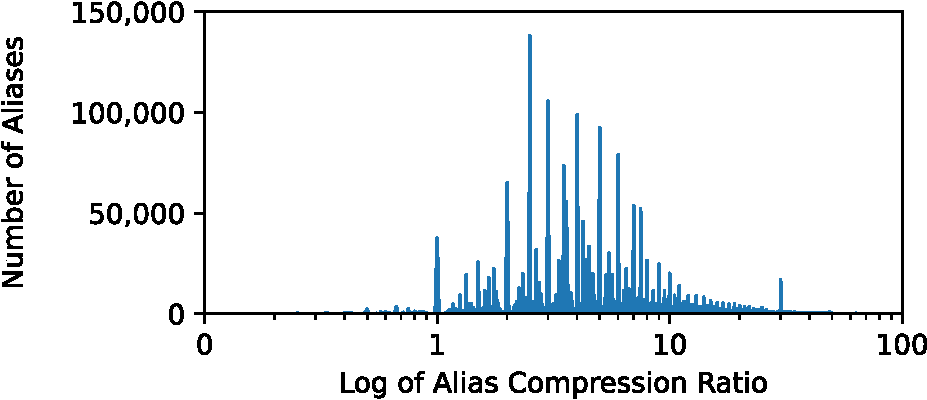
\includegraphics[width=0.95\columnwidth]{figures/compression.pdf}
    \caption{Distribution of alias compression ratios}
    \label{fig:compression}
\end{figure}

\paragraph{\bf Describing Actions}

A compression ratio less than 1 indicates an alias name that is longer than the value it aliases.
There are \num{26055} aliases (\per{1.18}) with names longer than their values.
Among them, we found many descriptive names, like
\begin{itemize}
    \item \verb|git-last-commit-message|
    \item \verb|docker_list_all_containers|
    \item \verb|generate_random_password|
\end{itemize}
and similar wordy descriptions of command invocations.

The two longest alias names we found are from joke definitions.
The first is \num{1772} characters long and is comprised of the letter `f' repeated \num{1053} times, followed by the letter `u' repeated 719 times.
It is an alias for the \verb|cat| command with a similarly named file as an argument.
The second longest alias name is a Swedish compound word of \num{131} characters,\footnote{Translating, roughly, to northwestern-glacier-artillery-flight-thrust-simulator-plant-equipment-maintenance-follow-up-systems-discussion-posts-preparation-works.} aliasing the \verb|ls| command.

\TODO names from dictionary

\paragraph{\bf Correcting Misspellings}

Aliases can be used to correct common misspellings of commands, like typing \verb|got| instead of \verb|git|.
While it is easy for the human eye to determine instances of these typographical errors, it is not as straightforward to formalize all different cases and to distinguish them from regular command shortcuts.
We opt for a conservative criterion (potentially underestimating the true extent of the phenomenon) that looks only at aliases whose names are of the same length as their aliased commands, with a string distance measure above an empirically determined threshold.
We surveyed and experimented with different distance measures~\cite{navarro:01} and decided on using the Damerau-Levenshtein algorithm~\cite{damerau:64}.
It is a robust measure that in addition to tracking the number of insertions, deletions, and substitutions between two strings, also captures the transposition of two characters, a common occurrence in misspelled commands.
We computed the distance measure for all applicable aliases, and determined empirically that a distance measure of 2 seems like a good threshold to decide whether or not an alias corrects a misspelling.
We found \num{9195} aliases (\per{0.42}) that serve as autocorrect rules, most commonly involving transposition (\verb|grpe| $\rightarrow$ \verb|grep|), case-sensitivity (\verb|Jupyter| $\rightarrow$ \verb|jupyter|), localization (\verb|pluralise| $\rightarrow$ \verb|pluralize|), and punctuation (\verb|docker-build| $\rightarrow$ \verb|docker_build|).

On the flip side, aliases are also used to disable autocorrect mechanisms.
The Z shell has built-in spelling correction, which can be selectively disabled using the \verb|nocorrect| command.
There are \num{7326} aliases (\per{0.33}) in our dataset disabling Z shell autocorrection for certain commands, most commonly the filesystem commands \verb|mv|, \verb|mkdir|, \verb|cp| and \verb|rm|.

\paragraph{\bf Bookmarking Locations}



\subsection{Changing}

\paragraph{\bf Substituting Commands}

\paragraph{\bf Overriding Defaults}

\paragraph{\bf Colorizing Output}

\paragraph{\bf Elevating Privilege}

\subsection{Composing}

\paragraph{\bf Building Tools}

\paragraph{\bf Transforming Data}

The most interesting shell operator is certainly the pipe (\verb`|`), since it creates an interface between two otherwise separate programs.
The pipe embodies the Unix philosophy of small tools doing one thing well, which can be connected together to accomplish more complex tasks.
\Cref{fig:flow} shows a flow diagram of the top 250 pipelines with three commands that make up at least \per{10} of one participating command's usage.
\TODO

\begin{figure*}[h]
	\centering    
	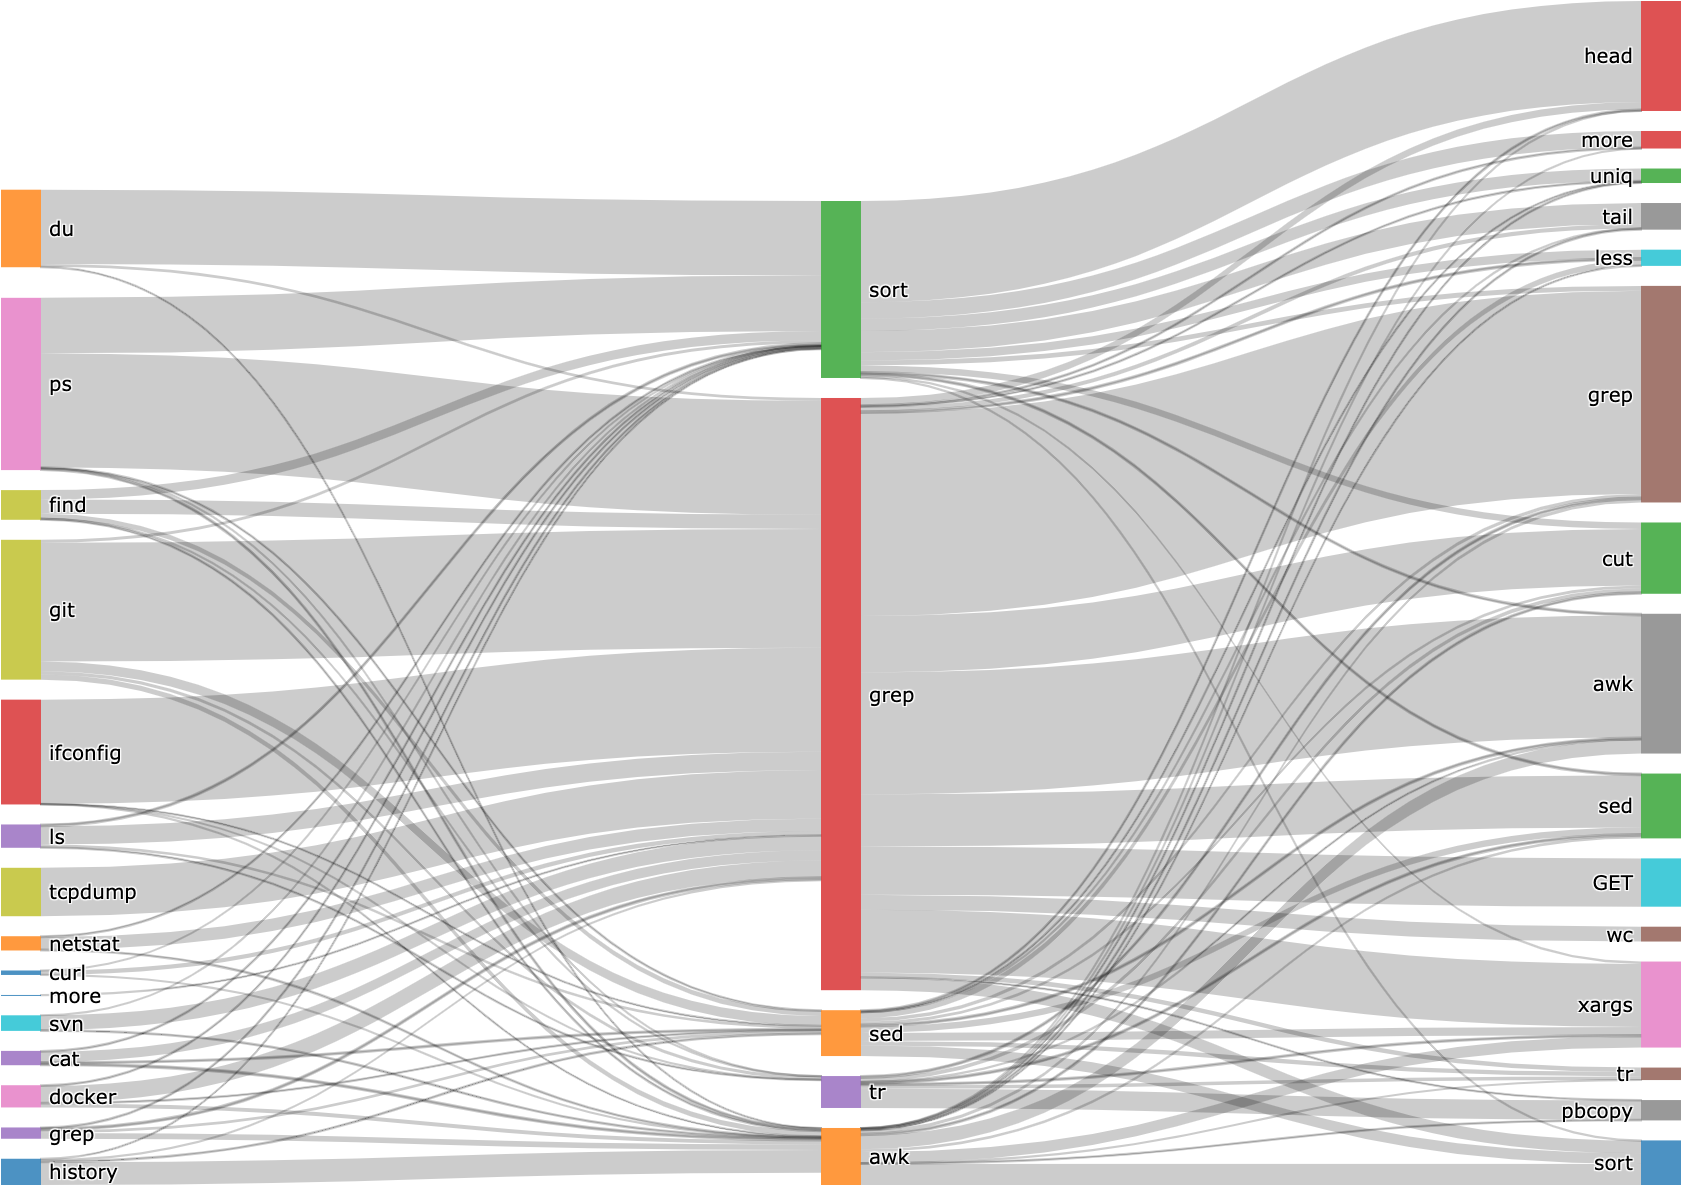
\includegraphics[width=0.9\linewidth]{figures/flow_250.png}
	\caption{Flow diagram for top 3-command pipelines}
	\label{fig:flow}
\end{figure*}


\paragraph{\bf Chaining Subcommands}

An interesting pattern found in aliases composed of multiple commands are chains of subcommand invocations.
For example, the package manager \verb|brew| has a subcommand \verb|update|, for updating the package database, and a subcommand \verb|upgrade|, for upgrading previously installed packages to the latest available versions.
\per{28.08} percent of all aliases involving the \verb|brew| command contain the composition
\begin{CVerbatim}
brew update && brew upgrade
\end{CVerbatim}
(sometimes with \verb|;| instead of \verb|&&|), with alias names like \verb|update|, \verb|brewup|, \verb|bup|, etc.
This pattern of repeated subcommand invocations can be found in \num{22062} aliases (\per{1}), and it is most prevalent among package managers, like \verb|brew|, \verb|apt-get|, \verb|npm| or \verb|gem|, mostly fulfilling roughly the same function as in the \verb|brew| example.

The command with the highest absolute number of aliases showing this pattern is \verb|git|, however, with \num{12063} occurrences (\per{3.89} of all aliases using \verb|git|).
Here, the uses are more varied:
\begin{CVerbatim}
alias commit='git add . && git commit -m'
alias whoops='git reset --hard && git clean -df'
alias gitpull='git stash && git pull && git stash pop'
\end{CVerbatim}
are just some examples of aliases combining the various \verb|git| subcommands.
